
The block diagram for the inner loop is shown in \fref{fig:hw_satellite_PD_inner}.
\controlbookfigure{0.8}
	{6_design_studies/figures/hw_satellite_PD_inner}
	{Block diagram for inner loop of satellite control}
	{fig:hw_satellite_PD_inner}
The closed loop transfer function from $\Theta^d$ to $\Theta$ is given by
\[
%\Theta(s) = \frac{\frac{k_{P_\theta}}{J_s}}{s^2 +\left(\frac{b+k_{D_\theta}}{J_s}\right)s+\left(\frac{k+k_{P_\theta}}{J_s}\right)} \Theta^d(s).
\Theta(s) = \frac{\frac{k_{P_\theta}}{J_s + J_p}}{s^2 +\left(\frac{k_{D_\theta}}{J_s + J_p}\right)s+\left(\frac{k_{P_\theta}}{J_s + J_p}\right)} \Theta^d(s).
\]
Therefore the closed loop characteristic equation is
\[
%\Delta_{cl}(s) = s^2 +\left(\frac{b+k_{D_\theta}}{J_s}\right)s+\left(\frac{k+k_{P_\theta}}{J_s}\right).
\Delta_{cl}(s) = s^2 +\left(\frac{k_{D_\theta}}{J_s + J_p}\right)s+\left(\frac{k_{P_\theta}}{J_s + J_p}\right).
\]
The desired closed loop characteristic equation is
\[
\Delta_{cl}^d(s) = s^2 + 2\zeta_{\theta}\omega_{n_\theta} s + \omega_{n_\theta}^2,
\]
where
\begin{align*}
\omega_{n_\theta} &= \frac{2.2}{t_{r_\theta}} = 2.2 \\
\zeta_{\theta} &= 0.9.
\end{align*}
Therefore
\begin{align*}
%k_{P_\theta} &= \omega_{n_\theta}^2J_s-k = 5.9 \\
k_{P_\theta} &= \omega_{n_\theta}^2(J_s + J_p) = 29.04 \\
%k_{D_\theta} &= 2\zeta_{\theta}\omega_{n_\theta} J_s-b = 7.727.
k_{D_\theta} &= 2\zeta_{\theta}\omega_{n_\theta}(J_s + J_p) = 23.76.
\end{align*}
The DC gain of the inner loop is given by
\[
%k_{DC_{\theta}} = \frac{k_{P_\theta}}{k+k_{P_\theta}} = 0.9752.
k_{DC_{\theta}} = 1.
\]

Replacing the inner loop by its DC gain, the block diagram for the outer loop is shown in \fref{fig:hw_satellite_PD_outer}.
\controlbookfigure{0.8}
	{6_design_studies/figures/hw_satellite_PD_outer}
	{Block diagram for outer loop of satellite attitude control}
	{fig:hw_satellite_PD_outer}
To find the closed loop transfer function from $\phi^d$ to $\phi$, follow the loop backwards from $\phi$ to obtain
\[
\Phi(s) = \left(\frac{\frac{b}{J_p}s+\frac{k}{J_p}}{s^2+\frac{b}{J_p}s+\frac{k}{J_p}}\right)\left[k_{DC_\theta}k_{P_\theta}(\Phi_r-\Phi)-k_{DC_\theta}k_{D_\theta}s\Phi\right].
\]
After some manipulation we get
\begin{multline}
\big[(J_p+bk_{DC_\theta}k_{D_\theta})s^2 + (b+bk_{DC_\theta}k_{P_\theta}+kk_{DC_\theta}k_{D_\theta})s 
	 + (k+kk_{DC_\theta}k_{P_\theta})\big]\Phi \\ = \left[bk_{DC_\theta}k_{P_\theta}s+kk_{DC_\theta}k_{P_\theta}\right]\Phi_r,
\end{multline}
which results in the monic transfer function
\[
\Phi(s)=\frac{\left(\frac{bk_{DC_\theta}k_{P_\theta}}{J_p+bk_{DC_\theta}k_{D_\theta}}\right)s+\left(\frac{kk_{DC_\theta}k_{P_\theta}}{J_p+bk_{DC_\theta}k_{D_\theta}}\right)}{s^2 + \left(\frac{b+bk_{DC_\theta}k_{P_\theta}+kk_{DC_\theta}k_{D_\theta}}{J_p+bk_{DC_\theta}k_{D_\theta}}\right)s + \left(\frac{k+kk_{DC_\theta}k_{P_\theta}}{J_p+bk_{DC_\theta}k_{D_\theta}}\right)} \Phi_r.
\]
The desired closed loop characteristic equation for the outer loop is
\[
\Delta_{cl}^d(s) = s^2 + 2\zeta_{\phi}\omega_{n_\phi} s + \omega_{n_\phi}^2,
\]
where
\begin{align*}
t_{r_\phi} &= 10~t_{r_\theta} = 10 \\
\omega_{n_\phi} &= \frac{2.2}{t_{r_\phi}} = 0.22 \\
\zeta_{\phi} &= 0.9.
\end{align*}
Therefore the gains $k_{P_\phi}$ and $k_{P_\theta}$ satisfy
\begin{align*}
\frac{k+kk_{DC_\theta}k_{P_\theta}}{J_p+bk_{DC_\theta}k_{D_\theta}} &= \omega_{n_\phi}^2 \\
\frac{b+bk_{DC_\theta}k_{P_\theta}+kk_{DC_\theta}k_{D_\theta}}{J_p+bk_{DC_\theta}k_{D_\theta}} &= 2\zeta_{\phi}\omega_{n_\phi}.
\end{align*}
Expressing these equations in matrix form gives
\[
\begin{pmatrix} kk_{DC_\theta} & -J_pbk_{DC_\theta} \\ bk_{DC_\theta} & kk_{DC_\theta}-2bk_{DC_\theta}\zeta_\phi\omega_{n_\phi} \end{pmatrix}\begin{pmatrix}k_{P_\phi}\\k_{D_\phi}\end{pmatrix} = \begin{pmatrix} -k + J_p\omega_{n_\phi}^2 \\ -b + 2J_p\zeta_\phi\omega_{n_\phi} \end{pmatrix},
\]
implying that
\begin{align*}
%\begin{pmatrix}k_{P_\phi}\\k_{D_\phi}\end{pmatrix} = \begin{pmatrix} kk_{DC_\theta} & -J_pbk_{DC_\theta} \\ bk_{DC_\theta} & kk_{DC_\theta}-2bk_{DC_\theta}\zeta_\phi\omega_{n_\phi} \end{pmatrix}^{-1} \begin{pmatrix} -k + J_p\omega_{n_\phi}^2 \\ -b + 2J_p\zeta_\phi\omega_{n_\phi} \end{pmatrix} = \begin{pmatrix} -0.6168 \\ 0.9778 \end{pmatrix}
\begin{pmatrix}k_{P_\phi}\\k_{D_\phi}\end{pmatrix} &= \begin{pmatrix} kk_{DC_\theta} & -J_pbk_{DC_\theta} \\ bk_{DC_\theta} & kk_{DC_\theta}-2bk_{DC_\theta}\zeta_\phi\omega_{n_\phi} \end{pmatrix}^{-1} 
	\begin{pmatrix} -k + J_p\omega_{n_\phi}^2 \\ -b + 2J_p\zeta_\phi\omega_{n_\phi} \end{pmatrix} \\
	&= \begin{pmatrix} 0.7946 \\ 2.621 \end{pmatrix}
\end{align*}

The DC gain of the outer loop is given by
\[
%k_{DC_{\phi}} = \frac{kk_{DC_\theta}k_{P_\phi}}{k+kk_{DC_\theta}k_{P_\phi}} = -1.5093.
k_{DC_{\phi}} = \frac{kk_{DC_\theta}k_{P_\phi}}{k+kk_{DC_\theta}k_{P_\phi}} = 0.4428.
\]
%Since the DC gain of the outer loop is not equal to one, $\phi_r$ in \fref{fig:hw_satellite_PD_outer} must be pre-multiplied by $1/k_{DC_\phi}$.
Note that the DC gain of the outer loop is not equal to one, so there will be significant steady state error. To remedy this, a feedforward term can be used to ensure that $\theta$ and $\phi$ are made to be equal in steady state, resulting in an overall DC gain of one. This configuration is depicted in \fref{fig:hw_satellite_PD_outer_feedforward}. Feedforward control will be discussed in a later chapter.

\begin{figure}[hbt]
  \centering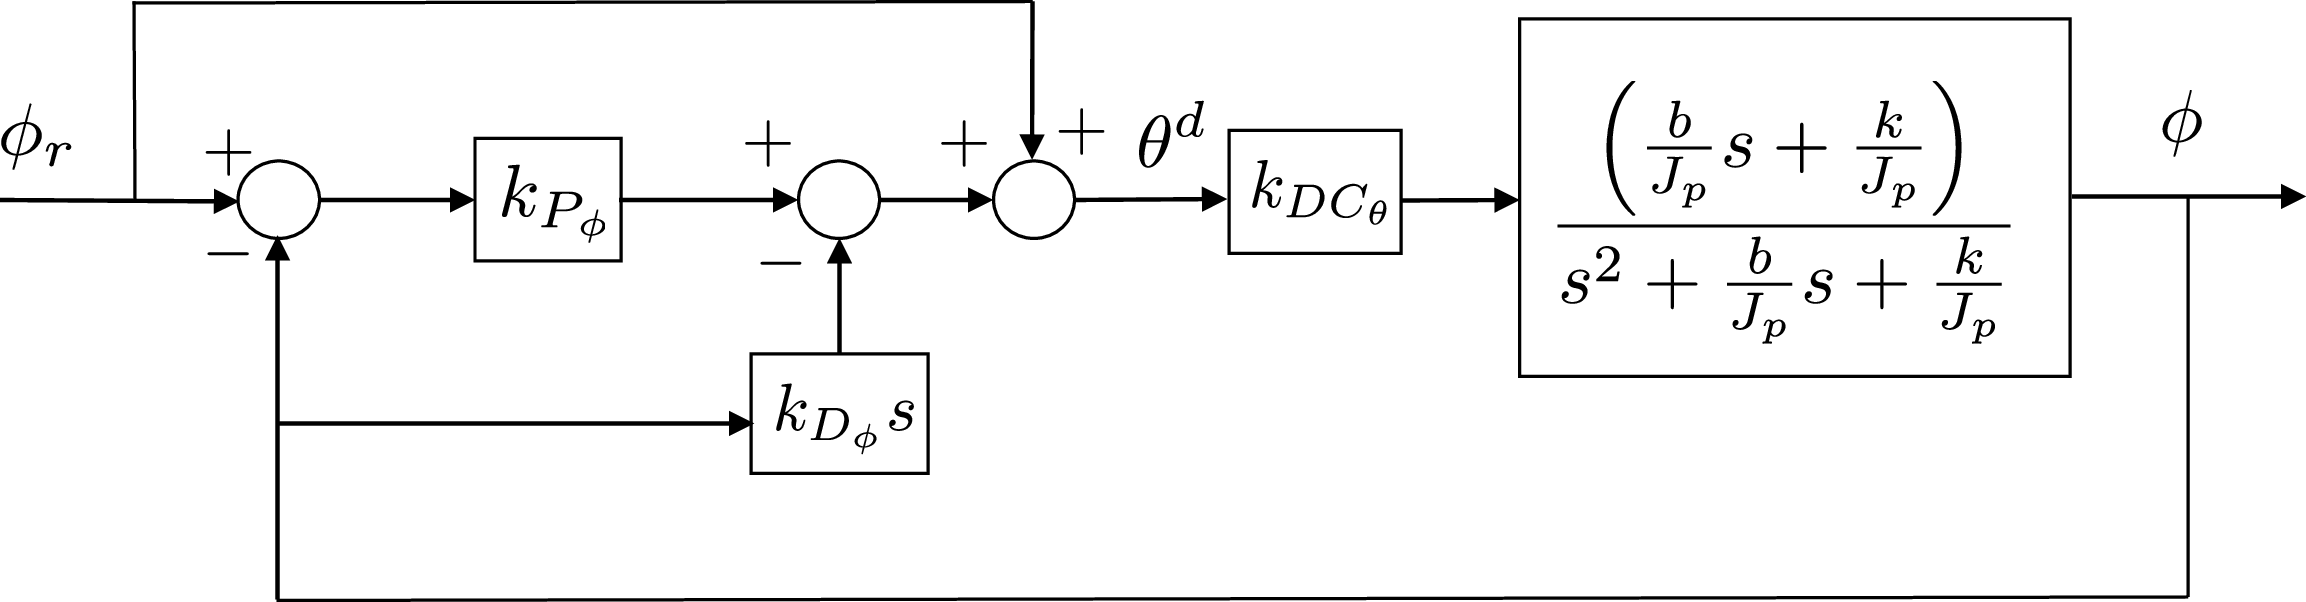
\includegraphics[width=0.8\textwidth]{6_design_studies/figures/hw_satellite_PD_outer_feedforward}
  \caption{Block diagram for outer loop of satellite attitude control with a feedforward term.}
  \label{fig:hw_satellite_PD_outer_feedforward} 
\end{figure}

A Python class that implements a PD controller using state feedback is shown below.
\lstinputlisting[language=Python, caption=satelliteController.py]{../control_book_public_solutions/_C_satellite/python/hw8/satelliteController.py}

Python code that implements the closed loop system is given below.
\lstinputlisting[language=Python, caption=satelliteSim.py]{../control_book_public_solutions/_C_satellite/python/hw8/satelliteSim.py}

Complete simulation code for Matlab, Python, and Simulink can be downloaded at \controlbookurl{http://controlbook.byu.edu}.
	
%A high-level Simulink diagram that implements the PD controller using state feedback is shown in Figure~\ref{fig:hw8_simulink_satellite}.
%\begin{figure}[hbt]
%  \centering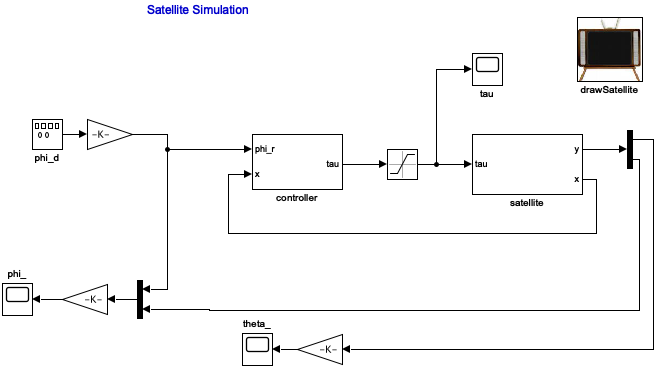
\includegraphics[width=0.8\textwidth]{6_design_studies/figures/hw8_simulink_satellite}
%  \caption{High level simulink diagram used for HW C.8}
%  \label{fig:hw8_simulink_satellite} 
%\end{figure}
%The Matlab/Simulink code for the controller is listed below.
%\lstinputlisting[language=Matlab, caption=satellite\_ctrl.m]{../control_book_public_solutions/_C_satellite/simulink/hw8/satellite_ctrl.m}

%The Matlab parameter file that computes the gains is listed below.
%\lstinputlisting[language=Matlab, caption=satelliteParamHW8.m]{../control_book_public_solutions/_C_satellite/simulink/hw8/satelliteParamHW8.m}


